%! Author = Len Washington III
%! Date = 2/4/24

% Preamble
\documentclass[title={Important Charts}]{com310notes}
\geometry{margin=0.06in}
\usepackage{colortbl}

% Packages

% Document
\begin{document}

\maketitle

%<*charts>
\begin{figure}[H]
	\centering
	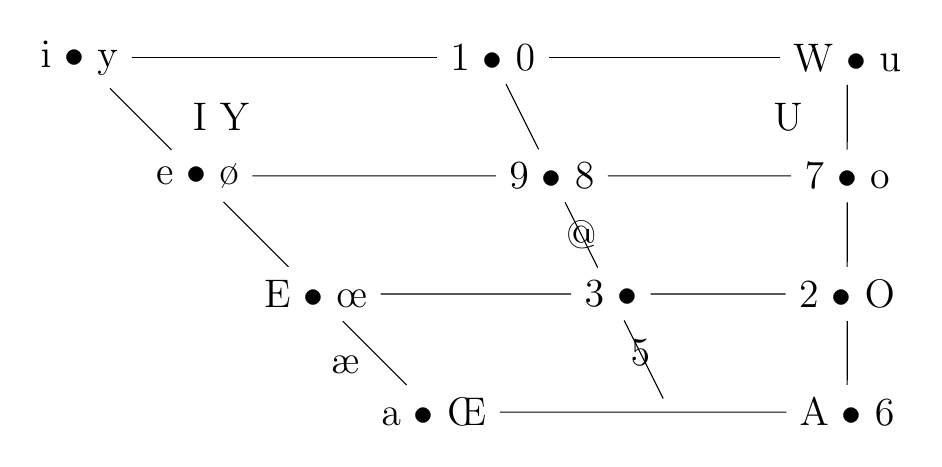
\begin{tikzpicture}[scale=1.5]
		\begin{scope}%\globalnodeset
			\Large
			\node (FrontClose) at (-0.5,0) {\ipa{i $\bullet$ y}};
			\node (FrontCloseMid) at (0.5,-1) {\ipa{e $\bullet$ \o}};
			\node (FrontOpenMid) at (1.5,-2) {\ipa{E $\bullet$ \oe}};
			\node (FrontOpen) at (2.5,-3) {\ipa{a $\bullet$ \OE}};

			\node (CentralClose) at (3,0) {\ipa{1 $\bullet$ 0}};
			\node (CentralCloseMid) at (3.5,-1) {\ipa{9 $\bullet$ 8}};
			\node (CentralOpenMid) at (4,-2) {\ipa{3 $\bullet$ \textcloserevepsilon}};
			\node (CentralOpen) at (4.5,-3) {};

			\node (BackClose) at (6,0) {\ipa{W $\bullet$ u}};
			\node (BackCloseMid) at (6,-1) {\ipa{7 $\bullet$ o}};
			\node (BackOpenMid) at (6,-2) {\ipa{2 $\bullet$ O}};
			\node (BackOpen) at (6,-3) {\ipa{A $\bullet$ 6}};

			\node (NearFrontClose) at (0.7, -0.5) {\ipa{I Y}};

			\node (NearFrontOpen) at (1.75, -2.6) {\ipa{\ae}};

			\node (CentralMid) at (3.75,-1.5) {\ipa{@}};

			\node (CentralOpenMidMid) at (4.25,-2.5) {\ipa{5}};

			\node (NearBackClose) at (5.5,-0.5) {\ipa{U}};
		\end{scope}
		\begin{scope}%\globalpathset
			\path (FrontClose) edge (CentralClose);
			\path (CentralClose) edge (BackClose);

			\path (FrontCloseMid) edge (CentralCloseMid);
			\path (CentralCloseMid) edge (BackCloseMid);

			\path (FrontOpenMid) edge (CentralOpenMid);
			\path (CentralOpenMid) edge (BackOpenMid);

			\path (FrontOpen) edge (BackOpen);

			\path (FrontClose) edge (FrontCloseMid);
			\path (FrontCloseMid) edge (FrontOpenMid);
			\path (FrontOpenMid) edge (FrontOpen);

			\path (CentralClose) edge (CentralCloseMid);
			\path (CentralCloseMid) edge (CentralOpenMid);
			\path (CentralOpenMid) edge (CentralOpen);

			\path (BackClose) edge (BackCloseMid);
			\path (BackCloseMid) edge (BackOpenMid);
			\path (BackOpenMid) edge (BackOpen);
		\end{scope}
	\end{tikzpicture}
	\caption{Vowels (Where symbols appear in pairs, the one to the right represents a rounded vowel.)}
	\label{fig:vowels}
\end{figure}

\begin{figure}[H]
	\centering
	\includegraphics[width=\textwidth]{vowels}
	\caption{Vowels (Where symbols appear in pairs, the one to the right represents a rounded vowel.)}
	\label{fig:}
\end{figure}

\begin{landscape}
	\begin{table}[H]
		\centering
		\begin{threeparttable}
			\caption{Consonants (Pulmonic)}
			\label{tab:ipa-table}
			\begin{tabular}{C{0.06\textwidth}|*{11}{C{0.03\textwidth} C{0.03\textwidth}|}}
				\hline
				& \multicolumn{2}{|C{0.06\textwidth}|}{bilabial} & \multicolumn{2}{|C{0.06\textwidth}|}{labio-dental} & \multicolumn{2}{|C{0.06\textwidth}|}{dental} & \multicolumn{2}{|C{0.06\textwidth}|}{alveolar} & \multicolumn{2}{|C{0.06\textwidth}|}{post-alveolar} & \multicolumn{2}{|C{0.06\textwidth}|}{retroflex} & \multicolumn{2}{|C{0.06\textwidth}|}{palatal} & \multicolumn{2}{|C{0.06\textwidth}|}{velar} & \multicolumn{2}{|C{0.06\textwidth}|}{uvular} & \multicolumn{2}{|C{0.06\textwidth}|}{pharyngeal} & \multicolumn{2}{|C{0.06\textwidth}|}{glottal}\\
				\hline
				Plosive (Stop) & 	p & b 	& 	& & 	\multicolumn{6}{|c|}{t d} 	& \ipa{\:t} & \ipa{\:d} & 	c & \textbardotlessj	& k & g & q & \ipa{\;G} & & \cellcolor{lightgray} & \ipa{P} & \cellcolor{lightgray} \\
				\hline
				Nasal (Stop) & & m & & \ipa{M} & \multicolumn{6}{|c|}{n} & & \ipa{\:n} & & \textltailn & & \ipa{N} & & \ipa{\;N} & \multicolumn{2}{|c|}{\cellcolor{lightgray}} & \multicolumn{2}{|c|}{\cellcolor{lightgray}} \\
				\hline
				Trill & & \ipa{\;B} & & & \multicolumn{6}{|c|}{r} & & & & & \multicolumn{2}{|c|}{\cellcolor{lightgray}} & & \ipa{\;R} & & & \multicolumn{2}{|c|}{\cellcolor{lightgray}} \\
				\hline
				Tap or Flap & & & & -- & \multicolumn{6}{|c|}{\ipa{R}} & & \ipa{\:r} & & & \multicolumn{2}{|c|}{\cellcolor{lightgray}} & & & & & \multicolumn{2}{|c|}{\cellcolor{lightgray}} \\
				\hline
				Fricative & \ipa{F} & \ipa{B} & \ipa{f} & \ipa{v} & \ipa{T} & \ipa{D} & \ipa{s} & \ipa{z} & \ipa{S} & \ipa{Z} & \ipa{\:s} & \ipa{\:z} & \c{c} & \ipa{J} & \ipa{x} & \ipa{G} & \ipa{X} & \ipa{K} & \textcrh & \ipa{Q} & \ipa{h} & \ipa{H}\\
				\hline
				(cental) approximant & & & & \ipa{V} & \multicolumn{6}{|c|}{\ipa{\*r}} & & \ipa{\:R} & & j & & \textturnmrleg & & & & & \multicolumn{2}{|c|}{\cellcolor{lightgray}} \\
				\hline
				lateral (approximant) & \multicolumn{2}{|c|}{\cellcolor{lightgray}} & \multicolumn{2}{|c|}{\cellcolor{lightgray}} & \multicolumn{6}{|c|}{l} & & \ipa{\:l} & & \ipa{L} & & \ipa{\;L} & & & \multicolumn{2}{|c|}{\cellcolor{lightgray}} & \multicolumn{2}{|c|}{\cellcolor{lightgray}}\\
				\hline
			\end{tabular}
			\begin{tablenotes}
				\small
				\item Where symbols appear in pairs, the one to the right represents a voiced consonant.
				Shaded areas denote articulations judged impossible.
			\end{tablenotes}
		\end{threeparttable}
	\end{table}
\end{landscape}
%</charts>

\end{document}